\documentclass[11pt]{article}
\usepackage[spanish]{babel}
\usepackage[utf8]{inputenc}
\usepackage{amsmath, amssymb}
\usepackage{geometry}
\usepackage{setspace}
\usepackage{enumitem}
\usepackage{graphicx}
\usepackage{xurl}
\usepackage{listings}

\geometry{letterpaper, margin=2cm}

\begin{document}
\begin{titlepage}
    \centering
    \vspace{2cm}
    {
\includegraphics[height=3.2cm]{../logo_unam.png}}
    \hfill
    {
\includegraphics[height=3.2cm]{../logo_fc.png}\par}
    \vspace{1cm}
    {\bfseries\LARGE UNIVERSIDAD NACIONAL AUTONOMA DE MÉXICO \par}
    \vspace{0.7cm}
    {\scshape\Large FACULTAD DE CIENCIAS \par}
    \vspace{1cm}
    {\itshape\Large Lenguajes de programación \par}
    \vspace{0.5cm}
    {\itshape\Large Semestre 2026-1 \par}
    \vspace{2cm}
    {\scshape\Huge Tarea 2 \par}
    \vspace{1cm}
    {\itshape\Large Fecha de entrega: 8 de septiembre de 2025 \par}
    \vspace{2cm}
    {\Large Autores: \par}
    \vspace{0.4cm}
    {\Large Escobar Gonzalez Isaac Giovani \hspace{1cm} 321336400 \par}
    {\Large Garduño Escobar Kevin Jonathan \hspace{0.5cm} 321070629 \par}
    {\Large Zaldivar Alanis Rodrigo \hspace{2.75cm} 424029605 \par}
\end{titlepage}
\section*{Instrucciones}
\noindent Resolver los siguientes ejercicios de forma clara y ordenada de acuerdo a los lineamientos de entrega de tareas disponibles en la página del curso.\\
\section*{Ejercicios}

\begin{enumerate}[leftmargin=0.8cm]

    \item Dadas las siguientes expresiones en la gramática \textit{WAE} dispuesta en sintaxis concreta, da la respectiva representación utilizando sintaxis abstracta por medio de los Árboles de Sintaxis Abstracta (ASA) correspondientes.\\
    En caso de no poder generar el árbol, justifica. \textbf{(1 puntos)}

    Para generar el árbol de sintaxis abstracta, procedemos primero a aplicar la función parse a las expresiones.
    \begin{enumerate}
        \item \{- 5 \{+ 17 \{+ 48 5\} \} \}\\
        \begin{lstlisting}
            > {parse {- 5 {+ 17 {+ 48 5}}}}
            > {sub {parse 5} {parse {+ 17 {+ 48 5}}}}
            > {sub {num 5} {add {parse 17} {parse {+ 48 5}}}}
            > {sub {num 5} {add {num 17}  {add {parse 48} {parse 5}}}}
            > {sub {num 5} {add {num 17}  {add {num 48} {num 5}}}}
        \end{lstlisting}
        \begin{center}
            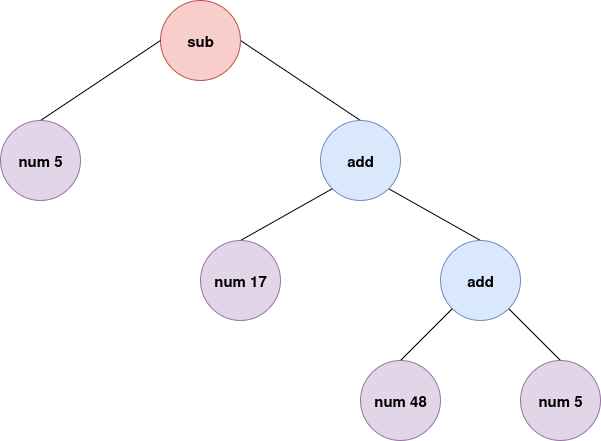
\includegraphics[height=6.5cm]{ASA.png}
        \end{center}

        \item \{- \{+ 30 \{+ 4 \} \} \}
        \begin{lstlisting}
            > {parse {- {+ 30 {+ 4 }}}}
            > Error!
        \end{lstlisting}
        El error producido se de debe a que, después de aplicar la primera línea de código, deja el - como sub y aplica parse al segundo elemento y al tercer elemento de la lista, sin embargo, en la expresión \{- \{+ 30 \{+ 4 \} \} \}, no existe un tercer elemento en la lista, por lo cuál el programa falla y no es una expresión bien formada en la gramática del lenguaje, por lo que esta expresión no tiene un árbol de sintaxis abstracta.
    \end{enumerate}

    \item Dadas las siguientes expresiones en la gramática \textit{WAE} dispuesta en sintaxis concreta, da la sintaxis abstracta correspondiente y realiza la sustitución que se indica. \textbf{(3 puntos)}
    \begin{enumerate}
        \item[a.] \begin{lstlisting}
e = {with {y {- 30 {- y z} } }
      {- 30 {+ y z } } }
(subst (parse e) 'y (id 'w))
        \end{lstlisting}
        Para convertir la expresión dada en la gramática \textit{WAE} en sintaxis concreta a abstracta, le aplicamos la función \texttt{parse} y se haría de la siguiente forma:
        \begin{lstlisting}
(parse e)
> {with {y {parse {- 30 {- y z}}}}
    {parse {- 30 {+ y z} } } }
> {with {y {sub {parse 30} {parse {- y z}}}}
    {parse {- 30 {+ y z} } } }
> {with {y {sub {num 30} {parse {- y z}}}}
    {parse {- 30 {+ y z} } } }
> {with {y {sub {num 30} {sub {parse y} {parse z}}}}
    {parse {- 30 {+ y z} } } }
> {with {y {sub {num 30} {sub {id y} {parse z}}}}
    {parse {- 30 {+ y z} } } }
> {with {y {sub {num 30} {sub {id y} {id z}}}}
    {parse {- 30 {+ y z} } } }
> {with {y {sub {num 30} {sub {id y} {id z}}}}
    {sub {parse 30} {parse {+ y z} } } }
> {with {y {sub {num 30} {sub {id y} {id z}}}}
    {sub {num 30} {parse {+ y z} } } }
> {with {y {sub {num 30} {sub {id y} {id z}}}}
    {sub {num 30} {add {parse y} {parse z} } } }
> {with {y {sub {num 30} {sub {id y} {id z}}}}
    {sub {num 30} {add {id y} {parse z} } } }
> {with {y {sub {num 30} {sub {id y} {id z}}}}
    {sub {num 30} {add {id y} {id z} } } }
        \end{lstlisting}
        Por lo tanto, la expresión queda:
        \begin{lstlisting}
e = {with {y {sub (num 30) {sub (id y) (id z)}}}
      {sub (num 30) {add (id y) (id z)} } }
        \end{lstlisting}
        Y expresión completa para aplicar la sustitución quedaría:
        \begin{lstlisting}
(subst {with {y {sub (num 30) {sub (id y) (id z)}}}
      {sub (num 30) {add (id y) (id z)}}} 'y (id 'w))
;; with -> (if (symbol=? y y)) = SI
> (with (y (subst {sub (num 30) {sub (id y) (id z)}} 'y (id 'w)))
    {sub (num 30) {add (id y) (id z)}})
> (with (y (sub (subst (num 30) 'y (id 'w)) (subst
    {sub (id y) (id z)} 'y (id 'w))))
    {sub (num 30) {add (id y) (id z)}})
> (with (y (sub (num 30) (subst {sub (id y) (id z)} 'y (id 'w))))
    {sub (num 30) {add (id y) (id z)}})
> (with (y (sub (num 30) (sub (subst (id y) 'y (id 'w))
    (subst (id z) 'y (id 'w)))))
    {sub (num 30) {add (id y) (id z)}})
;; id -> (if (symbol=? y y)) = SI
> (with (y (sub (num 30) (sub (id w) (subst (id z) 'y (id 'w)))))
    {sub (num 30) {add (id y) (id z)}})
;; id -> (if (symbol=? z y)) = NO
> (with (y (sub (num 30) (sub (id w) (id z))))
    (sub (num 30) (add (id y) (id z))))
        \end{lstlisting}
        La expresión final es:\\
        \boxed{\text{(with (y (sub (num 30) (sub (id w) (id z))))\\
    (sub (num 30) (add (id y) (id z))))}}

        \item[b.] e = \{+ a \{+ b \{- 32 57\} \} \}\\
        (subst (parse e) 'a (add (num 3) (num 4)))\\
        Aplicamos la función \texttt{parse} a la expresión:
        \begin{lstlisting}
(parse e)
> (add (parse a) (parse {+ b {- 32 57}} ))
> (add (id a) (parse {+ b {- 32 57}} ))
> (add (id a) (add (parse b) (parse {- 32 57}) ))
> (add (id a) (add (id b) (parse {- 32 57}) ))
> (add (id a) (add (id b) (sub (parse 32) (parse 57)) ))
> (add (id a) (add (id b) (sub (num 32) (parse 57)) ))
> (add (id a) (add (id b) (sub (num 32) (num 57)) ))
        \end{lstlisting}
        Por lo tanto, la expresión queda:
        \texttt{e = (add (id a) (add (id b) (sub (num 32) (num 57))))}
        Así, la expresión completa para aplicar la sustitución quedaría:
        \begin{lstlisting}
(subst (add (id a) (add (id b) (sub (num 32) (num 57))))
    'a (add (num 3) (num 4)))
> (add (subst (id a) 'a (add (num 3) (num 4)))
    (subst (add (id b) (sub (num 32) (num 57))) 'a (add (num 3) (num 4))))
;; id -> (if (symbol=? a a)) = SI
> (add (add (num 3) (num 4)) (subst (add (id b) (sub (num 32) (num 57)))
    'a (add (num 3) (num 4))))
> (add (add (num 3) (num 4)) (add (subst (id b) 'a (add (num 3) (num 4)))
    (subst (sub (num 32) (num 57)) 'a (add (num 3) (num 4)))))
;; id -> (if (symbol=? b a)) = NO
> (add (add (num 3) (num 4)) (add (id b))
    (subst (sub (num 32) (num 57)) 'a (add (num 3) (num 4)))))
> (add (add (num 3) (num 4)) (add (id b))
    (sub (subst (num 32)) (subst (num 57)) 'a (add (num 3) (num 4))))
> (add (add (num 3) (num 4)) (add (id b))
    (sub (num 32) (subst (num 57)) 'a (add (num 3) (num 4))))
> (add (add (num 3) (num 4)) (add (id b) (sub (num 32) (num 57))))
        \end{lstlisting}
        La expresión final es:\\
        \boxed{\text{(add (add (num 3) (num 4))
        (add (id b) (sub (num 32) (num 57))))}}
    \end{enumerate}
\newpage

    \item Convierte las siguientes expresiones usando la notación de índices de \textit{De Bruijn}.\textbf{(3 puntos)}
    \begin{lstlisting}
{with {v 2}
  {with {w 3}
    {with {x 4}
      {with {y {+ v {- w x} } }
        {with {z {with {v {+ w x } } v } }
          {+ y {with {w {- y z } } {- w x } } } } } } } }
    \end{lstlisting}

    \textbf{Solución:}

    \begin{lstlisting}
{with 2
  {with 3
    {with 4
      {with {+ <:2 0> {- <:1 0> <:0 0>} }
        {with {with {+ <:2 0> <:1 0> } <:0 0> }
          {+ <:1 0> {with {- <:1 0> <:0 0> } {- <:0 0> <:3 0> } } } } } } } }
    \end{lstlisting}


    \item Dadas las siguientes expresiones representadas mediante índices de \textit{De Bruijn}, obtén su respectiva versión usando los nombres de los identificadores de variables, iniciando por ”a”, ” b ”, ”c”, ”d”, ”e”, ”f ”.\textbf{(3 puntos)}

    \begin{lstlisting}
{multi-with {1 2 3 }
  {multi-with {4 5 6 }
    {with { {multi-with { {+ <:0 1> <:1 2>} {- <:1 1> <:0 0>} } 3 } }
      {with {<: 0 0>}
        {+ <:3 2> {+ <:2 1> {+ <:1 0> <:0 0>} } } } } } }
    \end{lstlisting}

    \textbf{Solución:}

    \begin{lstlisting}
{multi-with {{a 1} {b 2} {c 3} }
  {multi-with {{d 4} {e 5} {f 6} }
    {with { g {multi-with {{+ e c}{- b d}} 3} }
      {with { h g}
        {+ c {+ e {+ g h} } } } } } }
    \end{lstlisting}

\end{enumerate}

\section*{Bibliografía:}


\end{document}
